\section{Preliminary design}
	Based on the selected concept the simplest body diagram has been created in order to start the dimensioning of the main elements of the structure. Considering the possible practical implementation of the system, the symbolic representation of the moving frame has been made (figure \ref{fig:freebodydiagramframe}).
	
	\begin{figure}[bht]
		\centering 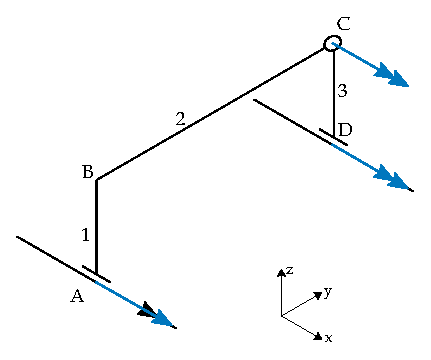
\includegraphics{preliminary-a}
		\caption{schematic representation of the moving frame supporting the arm; blue arrows are describes the rotational degree of freedom left by the joints. \textbf{FIGURA DA MODIFICARE}}
		\label{fig:freebodydiagramframe}
	\end{figure}
	
	The design involves a main elevated track (body 2) supported by two vertical supporting beams (body 1 and 3); the connection between body 1 and 2 has done by a full joint with 6 degrees of constrain while the connection of the track with the other support is done by a hinge that leaves free the rotation over the global $x$ axis. The two vertical supports can slide on two parallel tracks and the associated prismatic joints constraints 4 degrees of freedom each, leaving the system free to slide and accommodating rotation over the global $x$ axis. The choice of the joints is made in order to make the system immune to misalignment of the tracks (in particular considering their non-perfect parallelism and the fact that they can't be coplanar).
	
	As simplification on both the geometry and the load we consider:
	\begin{itemize}
		\item on the elevated track the loads transferred by the working appendix are modelled as a pure vertical force $P$ (mainly related to the approximate weight) and a torque $T$ that model's the one due to the plower; the eccentricities of both forces are in this case neglected and the application of application of both actions is placed at a distance $\xi$ refered to the local coordinate $z_2$ of the elevated track;
		
		\item the vertical supports are equally dimensioned and present a characteristic height $H$; the elevated track connecting them has length $L$;
		
		\item referring to figure \te, the action associated to the joint in $B$ aren't described (the theoretical connection of bodies 1 and 2 should behave as a single element), however the practical final result will imply the connection of two separate beams.	
		
	\end{itemize}

	Chosen the two hyper-static variable $X_1,X_2$ to reduce the problem to an isostatic one the parametric definitions of the reaction forces are
	\[ R_{Az} = \frac {L-\xi}L P \qquad M_{Ay} = -X_2 \qquad R_{Cz} = \frac \xi L P \qquad M_{Cy} = X_2 \] \[ M_{Cz} = T - X_1 \qquad R_{Dz} = \frac \xi L P \qquad M_{Dz} = T - X_1 \]
	The other actions ($R_{Ay},R_{Cx}, R_{Cy}, R_{Dy}$) are instead identically null. To solve the hyper-static problem the Castigliano's theorem has been used, computing the elastic energy $U_e$ of the structure neglecting shear loads:
	\[ U_e = \sum_{i=1}^3 \int_0 ^{L_i}  \left( \frac{N_i^2}{2EA_i} + \frac{M_{x,i}^2}{2 EI_{xx,i}} + \frac{M_{y,i}^2}{2 E I_{yy,i}} + \frac{M_{z,i}^2}{2G J_{t,i}}  \right)\, dz \]
	Assuming the generalized displacement related to the hyper-static variables as null, solving the equations $\partial U_e / \partial X_1 = 0$ and $\partial U_e/\partial X_2$ determines the solutions
	\[ X_1 = \frac T 2 \qquad \qquad \qquad X_2 = 0 \]
	
	
	In this preliminary design phase in order to over-estimate the loads the the frame should bear a weight $P = 196 N$ is considered (associated to a weight of about $20kg$ that relates to all the carried equipment on the moving arm including batteries and water tank) and a value of torque $T = 0.8 N\cdot m$ associated to the maximum force due to the plower that's transmitted on the frame itself. As geometrical dimension the considered length of the rail is $L=3m$ supported to a height $H = 0.7m$.
	
	\paragraph{Choice of the standard beams} With the preliminary design model described, different solutions can be found looking from various vendors present in the marker. In particular for the project main reference has been made to the Parker IPS catalogue \cite{parker-ds} due to the high availability of accessories components, however similar product can be found by other vendors (as group we also evaluated 8020 \cite{8020-ds} and Tslots by Bonnel Aluminum \cite{tslot-ds}).
	
	Data-sheets presents information about the section area $A$ and second moments of area $I_{xx},I_{yy}$ respect the primary axes, however no information is given for the torsional rigidity $J_t$ and so the related component is in the calculation neglected. Considering the lack in the consideration of both shear and torsion and the imprecise geometry and load conditions, the chosen product must withstand the mentioned load with a safety-factor $\phi$ of at least 6.
	
	After an iterative process, the standard section in table \ref{tab:beamchoice} are chosen withstanding a minimum safety factor $\phi = 9.12$ considering only axial and bending loads.
	
	\begin{table}[bt]
	\rule{\linewidth}{2pt}
	\caption{selected beams section chosen from the Parker IPS catalogue \cite{parker-ds} and related main properties (area, moments of inertia and weight per unit length).}
	\label{tab:beamchoice}
	\rule{\linewidth}{1pt} \vspace{0mm}	
	
	\begin{center}
		\begin{tabular}{p{3cm} | c c c c  |  l }
			& Area & \multicolumn{2}{c}{Moments of inertia} & Weight \\
			Usage & $A [cm^2]$ & $I_{xx} [cm^4]$ & $I_{yy} [cm^4]$ & $p [kg/m]$ & Product code \\ \hline
			track & 9.29 & 14.26 & 14.26 & 2.53 & \texttt{11-040} \\
			supports & 5.20 & 8.27 & 8.27 & 1.41 & \texttt{10-540} \\
		\end{tabular}
	\end{center}
	
	\vspace{3mm}
	\rule{\linewidth}{1pt}
	{\scriptsize
		\begin{multicols}{2}
		\begin{center}
			\includegraphics[height=2cm]{11-040}	\\		
			\includegraphics[height=2cm]{10-540}
		\end{center}
		\end{multicols}
		Representation of the sections for the track beam (on the left) and the supports (right).
	}	
	
	\rule{\linewidth}{2pt}
	
\end{table}
	
	

	
	
	
	
	
	
	
	
	
	
	
	
	
	
	
	
	
	
	
	
	
	
	
	
	
	
	
	
	
	
	
	